\section{The Galton--Watson process}
\label{sec:gw}

Replace the exponential clock of \cref{sec:lbd} by a generational one and the
birth--death process becomes the Galton--Watson process: a discrete-time, discrete-state
Markov chain in which every member of the population independently either reproduces or
dies at each generational increment. Formulated by Francis Galton and Henry Watson in
the late nineteenth century, it remains the most basic model of stochastic branching
\cite{Athreya1972,Harris1963}, and it is the setting in which the conditioning arguments
of this chapter are cleanest.

Let each individual produce, at the end of its life and independently of every other, a
number of offspring distributed as the \rv{} $\xi$, with
\begin{equation*}
\pr{\xi = k} = p_k,\qquad k=0,1,2,\dots,
\end{equation*}
and write $\mu = \mean{\xi}$ for the mean family size. Let $\zz_n$ be the number of
individuals in generation $n$, started from a single progenitor, $\zz_0=1$. Conditioning
on the previous generation and using the tower property,
\begin{equation*}
\mean{\zz_{n+1}} = \mean{\mean{\zz_{n+1}\mid\zz_n}} = \mean{\mu\,\zz_n} = \mu\,\mean{\zz_n},
\end{equation*}
so $\mean{\zz_n} = \mu^n$. When $\mu<1$ the expected population decays geometrically and
$\pr{\zz_n=0}\to1$: extinction is certain. The mean alone settles the question in that
regime, and nothing else in this chapter would be needed if the mean were all one wanted.

Generating functions supply the rest. Write $\phi(z) = \mean{z^{\xi}}$ for the offspring
\pgf{} and $u_n = \pr{\zz_n=0}$ for the probability of extinction by generation $n$.
Generation $n$ is the union of the families produced by the individuals of generation
$n-1$, and those families are independent and identically distributed, so
\cref{eq:pgfindep} gives $\mean{z^{\zz_n}\mid\zz_{n-1}=m} = \phi(z)^m$ and hence
$\phi_n(z) = \mean{\phi(z)^{\zz_{n-1}}} = \phi_{n-1}\bigl(\phi(z)\bigr)$. Iterating, the
\pgf{} of $\zz_n$ is the $n$-fold composition
\begin{equation}
\label{eq:phicomp}
\phi_n(z) = \mean{z^{\zz_n}}
= \underset{n\ \text{times}}{\underbrace{\phi\lrb{\phi\lrb{\cdots\phi\lrb{z}}}}},
\end{equation}
and evaluating at $z=0$ gives the iteration on which almost everything below depends,
\begin{equation}
\label{eq:iterPGF}
u_{n+1} = \phi(u_n),\qquad u_0=0 .
\end{equation}
Extinction of a branching process is a fixed-point problem for a one-dimensional map.

\subsection{Death or division}
\label{sec:deathordivision}

From here on we specialise to the binary --- or \emph{simple} --- case, in which an
individual either divides into two or dies:
\begin{align*}
p_2 &= p &&\text{(division)},\\
p_0 &= 1-p &&\text{(death)},\\
p_i &= 0 &&\forall\, i\neq0,2 .
\end{align*}
The mean family size is then $\mu = 2p$, and the expected population descended from a
single ancestor is
\begin{equation}
\label{eq:meanZn}
\mean{\zz_n} = (2p)^n .
\end{equation}
The process is \emph{subcritical} when $2p<1$, \emph{critical} when $p=\tfrac12$, and
\emph{supercritical} when $2p>1$. \Cref{fig:gwvis} shows realisations on either side of
the critical point, drawn as genealogies.

\begin{figure}[ht]
\centering
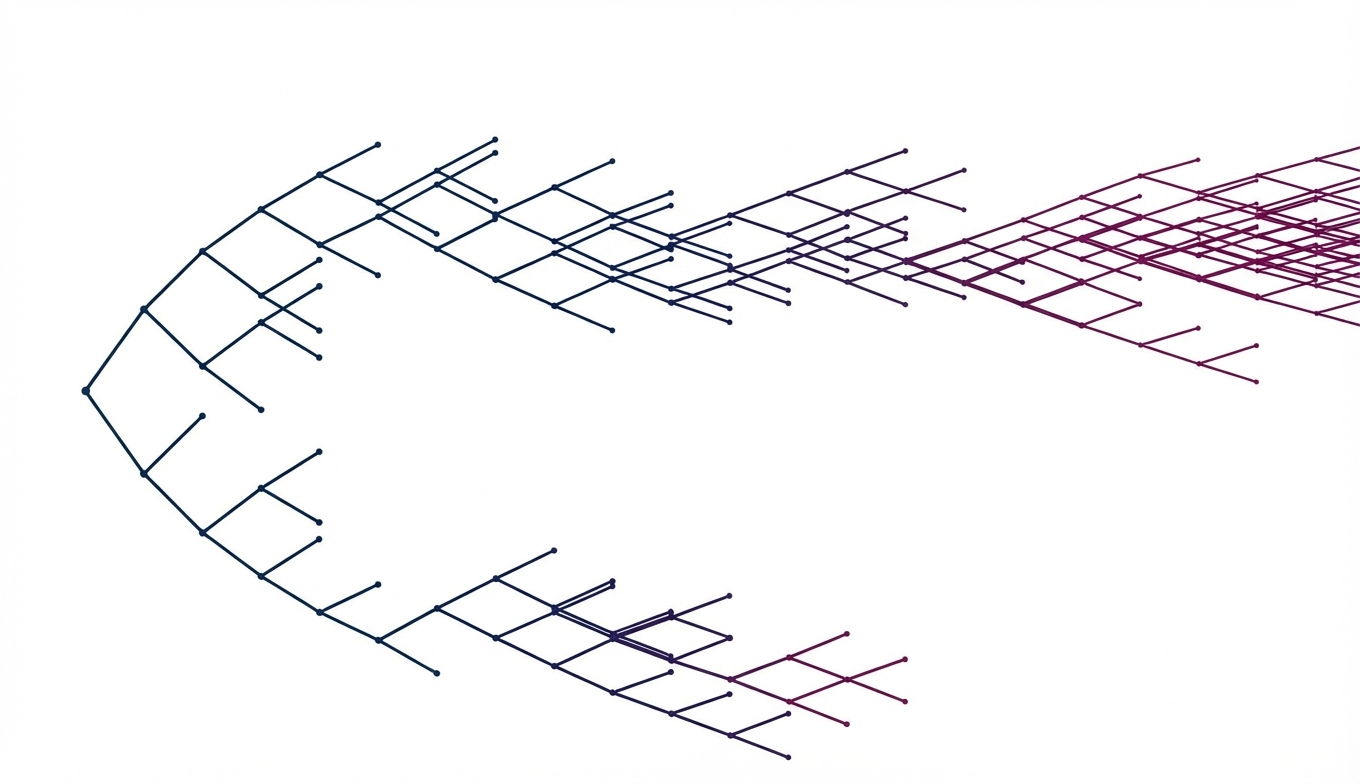
\includegraphics[width=0.78\textwidth]{figures/IMG_ch3/simpleGWvis.png}\\[6pt]
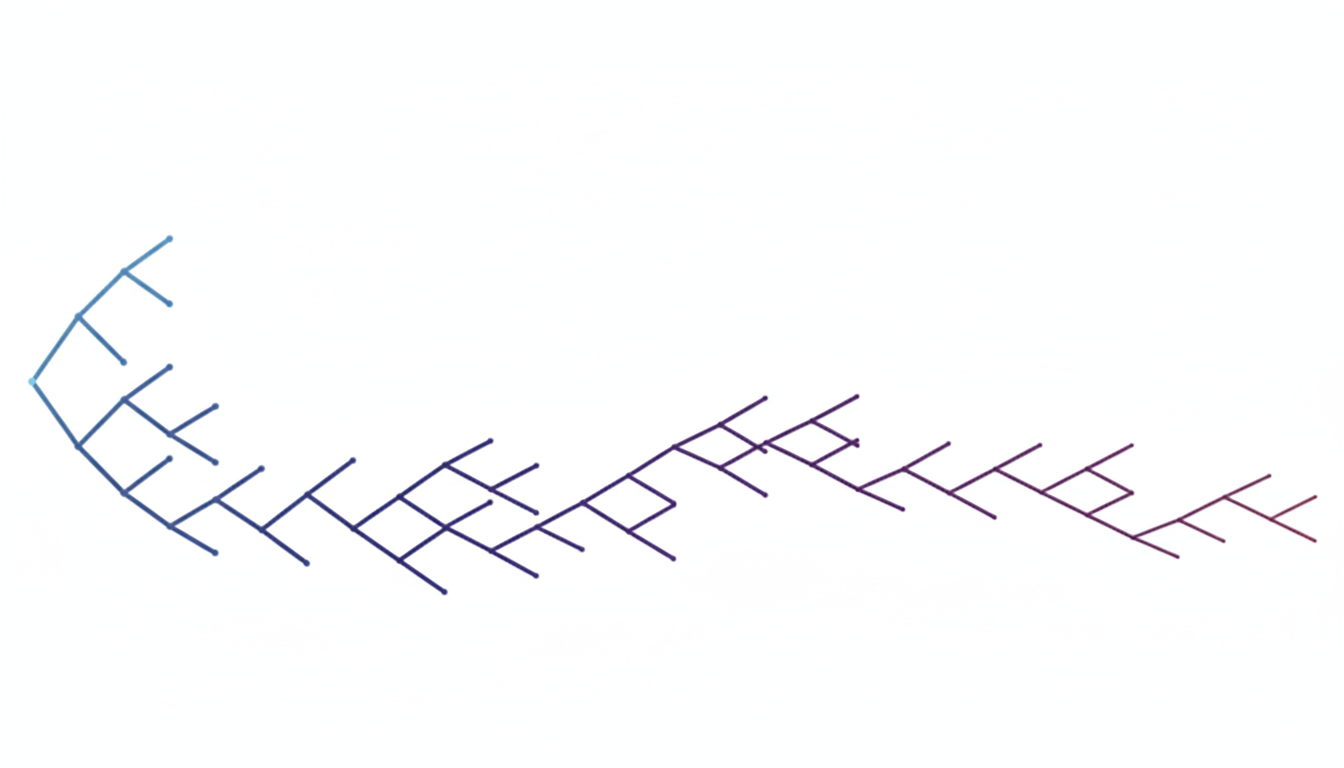
\includegraphics[width=0.78\textwidth]{figures/IMG_ch3/subGWvis.png}
\caption{Realisations of the simple Galton--Watson process, drawn as genealogies with
generation increasing to the right and colour encoding generation number. Top:
supercritical, $p=0.58$, in which the number of lines grows without bound. Bottom:
subcritical, $p=0.47$, in which the identical construction terminates. The two panels
differ only in the value of $p$.}
\label{fig:gwvis}
\end{figure}

\noindent
The offspring \pgf{} is a quadratic,
\begin{equation}
\label{eq:pgfbinary}
\phi(z) = \mean{z^{\zz_1}} = pz^2 + (1-p),
\end{equation}
so that \cref{eq:iterPGF} reads
\begin{equation}
\label{eq:unIter}
u_{n+1} = p\,u_n^2 + 1-p .
\end{equation}
The recursion admits a direct reading, which is worth having because it is the reading
that generalises. If the founder dies at its first step, with probability $1-p$, then
extinction has already occurred. If instead it divides, with probability $p$, then
extinction by generation $n+1$ requires each of the two fresh lineages to die out within
its own $n$ generations, and those lineages are independent, so that event has
probability $u_n^2$.

It is more convenient to track the complement,
\begin{equation*}
S_n = 1-u_n = \pr{\zz_n>0},
\end{equation*}
the probability that the process is still alive at generation $n$. Substituting
$u_n = 1-S_n$ into \cref{eq:unIter} and simplifying,
\begin{equation}
\label{eq:SnIter}
S_{n+1} = 2pS_n - pS_n^2,\qquad S_0=1 .
\end{equation}
A population cannot return from extinction, so $u_n$ is non-decreasing and bounded above
by $1$; equivalently $S_n$ is non-increasing and bounded below by $0$, and therefore
converges to some $S_\infty\in[0,1]$. The recursion \cref{eq:SnIter} is the central
object of \cref{sec:qsd,sec:small,sec:Ap}, and every difficulty encountered there is a
difficulty about this one quadratic map.

\subsection{Certainty of extinction}
\label{sec:certainty}

Since $S_n$ converges, its limit must be a fixed point of \cref{eq:SnIter}. Setting
$S_{n+1}=S_n=S_\infty$,
\begin{equation*}
S_\infty = 2pS_\infty - pS_\infty^2
\qquad\Longleftrightarrow\qquad
p\,S_\infty\lrb{S_\infty + \tfrac1p - 2} = 0,
\end{equation*}
with roots
\begin{equation*}
S_\infty = 0
\qquad\text{and}\qquad
S_\infty = 2-\frac1p = \frac{2p-1}{p}.
\end{equation*}
For $p<\tfrac12$ the second root is negative and carries no probabilistic meaning, so
the only admissible limit is $S_\infty=0$ and extinction is certain. At $p=\tfrac12$ the
two roots collide at the origin and extinction remains certain, now marginally. For
$p>\tfrac12$ a positive root appears at $S_\infty=(2p-1)/p$, and it is this root that is
attained: the process survives forever with positive probability. \Cref{fig:phase_transition}
displays the transition as a change in the stability of the origin.

\begin{figure}[htbp]
    \centering
    \begin{subfigure}[b]{0.31\textwidth}
        \centering
        \begin{tikzpicture}
            \begin{axis}[myplotstyle]
                \addplot[blue, thick] {2*0.3*x - 0.3*x^2};
                \addplot[black!45, dashed] {x};
                \addplot[only marks, mark=*, red, mark size=1.6pt] coordinates {(0,0)};
            \end{axis}
        \end{tikzpicture}
        \caption{Subcritical ($p = 0.3$)}
    \end{subfigure}
    \hfill
    \begin{subfigure}[b]{0.31\textwidth}
        \centering
        \begin{tikzpicture}
            \begin{axis}[myplotstyle]
                \addplot[blue, thick] {2*0.5*x - 0.5*x^2};
                \addplot[black!45, dashed] {x};
                \addplot[only marks, mark=*, red, mark size=1.6pt] coordinates {(0,0)};
            \end{axis}
        \end{tikzpicture}
        \caption{Critical ($p = 0.5$)}
    \end{subfigure}
    \hfill
    \begin{subfigure}[b]{0.31\textwidth}
        \centering
        \begin{tikzpicture}
            \begin{axis}[myplotstyle]
                \addplot[blue, thick] {2*0.74*x - 0.74*x^2};
                \addplot[black!45, dashed] {x};
                \addplot[only marks, mark=*, red, mark size=1.6pt] coordinates {(0,0) (0.64865,0.64865)};
            \end{axis}
        \end{tikzpicture}
        \caption{Supercritical ($p = 0.74$)}
    \end{subfigure}

    \vspace{10pt}
    \begin{subfigure}[b]{0.55\textwidth}
    \centering
    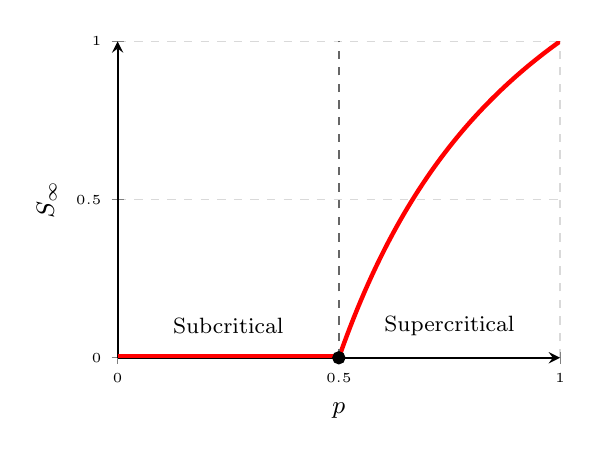
\begin{tikzpicture}
        \begin{axis}[
            width=7.2cm, height=5.6cm,
            axis lines=left,
            xlabel={$p$}, ylabel={$S_\infty$},
            xmin=0, xmax=1, ymin=0, ymax=1,
            xtick={0,0.5,1}, ytick={0,0.5,1},
            grid=major, grid style={dashed, gray!30}, thick,
            label style={font=\small}, tick label style={font=\tiny}
        ]
            \addplot[red, ultra thick, domain=0:0.5] {0.004};
            \addplot[red, ultra thick, domain=0.5:1, samples=120] {(2*x-1)/x};
            \draw[dashed, black!60] (axis cs:0.5,0) -- (axis cs:0.5,1);
            \node[font=\footnotesize] at (axis cs:0.25, 0.10) {Subcritical};
            \node[font=\footnotesize] at (axis cs:0.75, 0.10) {Supercritical};
            \addplot[only marks, mark=*, mark size=2pt, black] coordinates {(0.5,0)};
        \end{axis}
    \end{tikzpicture}
    \caption{The transition in $S_\infty$}
    \end{subfigure}

    \caption{Steady states of the survival recursion \cref{eq:SnIter}. Panels (a)--(c)
    plot the map $S\mapsto2pS-pS^2$ in blue against the diagonal, dashed; fixed points
    are the intersections, marked in red. Below and at criticality the origin is the only
    fixed point in $[0,1]$ and it attracts, so extinction is certain. At $p=\tfrac12$ the
    map is tangent to the diagonal at the origin. For $p>\tfrac12$ the origin turns
    repelling and a stable positive fixed point $S_\infty=(2p-1)/p$ separates from it,
    traced in panel~(d). The survival probability is identically zero below $p=\tfrac12$
    and rises continuously above it.}
    \label{fig:phase_transition}
\end{figure}

\subsection{Criticality: a power law and an infinite expected lifetime}
\label{sec:criticalcase}

The critical case sits awkwardly between the two others and deserves separate treatment.
At $p=\tfrac12$ the expected population is constant, $\mean{\zz_n}=1^n=1$ for every $n$,
and yet extinction is certain. The two facts are reconciled by the expected
\emph{lifetime} being infinite: rare realisations survive for enormous times and grow
enormously large, and they do so at exactly the rate needed to hold the mean at one.
Demonstrating this is worthwhile in itself, and the same calculation supplies the
asymptotics of $S_n$ that \cref{sec:Ap} will need.

Let
\begin{equation*}
T = \inf\{n : \zz_n=0\}
\end{equation*}
be the extinction time, so that the process passes through generations $0,1,\dots,T-1$
and is dead at $T$. Writing $T$ as a sum of indicators and taking expectations term by
term --- legitimate because every term is non-negative ---
\begin{equation}
\label{eq:ETsumSn}
T = \sum_{n=0}^{\infty}\mathbf{1}_{\{T>n\}},
\qquad
\mean{T} = \sum_{n=0}^{\infty}\pr{T>n} = \sum_{n=0}^{\infty}\pr{\zz_n>0} = \sum_{n=0}^{\infty}S_n .
\end{equation}
The question is therefore how fast $S_n$ decays at criticality.

Setting $p=\tfrac12$ in \cref{eq:SnIter} removes the linear term entirely and leaves
\begin{equation*}
S_{n+1}-S_n = -\tfrac12 S_n^2 .
\end{equation*}
Once $n$ is large the unit generational increment is small compared with the scale on
which $S_n$ varies, so the difference on the left is well approximated by a derivative:
\begin{equation*}
\dda{S}{n} = -\tfrac12 S^2,
\qquad\text{with general solution}\qquad
S(n) = \frac{2}{n+\text{const}} .
\end{equation*}
The approximation is heuristic --- it is the continuum limit of a difference equation,
and its constant of integration is not determined by it --- but the decay rate it
predicts is correct:
\begin{equation}
\label{eq:twoovrn}
S_n \sim \frac{2}{n}\qquad(n\to\infty),
\end{equation}
as the simulations of \cref{fig:power_law}(a) confirm. Substituting into
\cref{eq:ETsumSn}, the tail of the sum behaves like twice the harmonic series,
\begin{equation*}
\mean{T} = \sum_{n=0}^{\infty}S_n \sim \sum_{n=1}^{\infty}\frac{2}{n},
\end{equation*}
which diverges (\cref{fig:harmonic}). Since every $S_n$ is positive, $\mean{T}=\infty$:
the expected lifetime of the critical Galton--Watson process is infinite even though
extinction occurs with probability one.

\begin{figure}[H]
    \centering
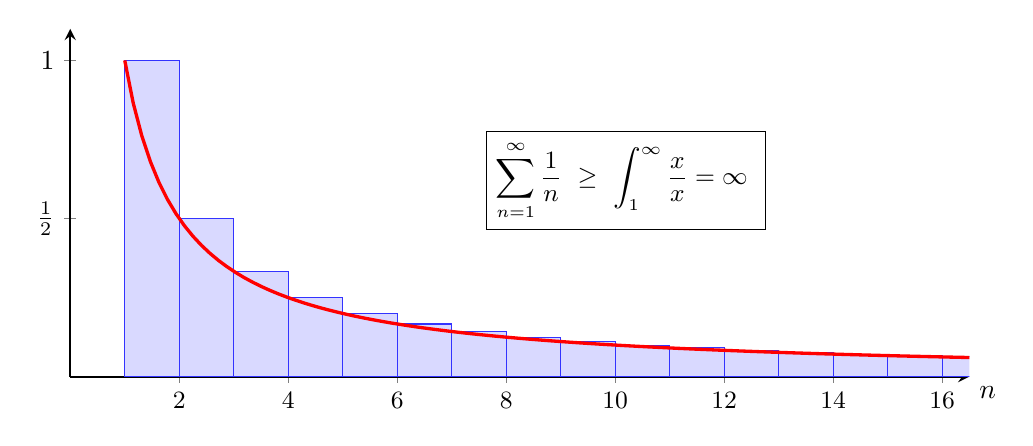
\begin{tikzpicture}
    \begin{axis}[
        axis lines = middle,
        xmin = 0, xmax = 16.5, ymin = 0, ymax = 1.1,
        xlabel = {$n$},
        xtick = {2,4,6,8,10,12,14,16},
        ytick = {0.5, 1}, yticklabels = {$\frac{1}{2}$, $1$},
        axis line style = {thick},
        width = 13cm, height = 6cm,
        every axis x label/.style={at={(current axis.right of origin)}, anchor=north west},
        xticklabel style={font=\small},
    ]
        \addplot[fill=blue!15, draw=blue!80, ybar interval, samples at={1,2,...,17}] {1/x} \closedcycle;
        \addplot[red, domain=1:16.5, samples=100, very thick] {1/x};
        \node[draw, fill=white, align=left, font=\small] at (axis cs: 10.2, 0.62) {
            $\displaystyle \sum_{n=1}^{\infty} \frac{1}{n} \ \ge\ \int_{1}^{\infty} \frac{\dd x}{x} = \infty$
        };
    \end{axis}
\end{tikzpicture}
\caption{Divergence of the harmonic series. Each blue rectangle has area $1/n$ and
contains the region under the red curve $1/x$ on $[n,n+1]$, so the areas sum to more
than $\int_1^\infty x^{-1}\dd x = \infty$. Because $S_n\sim2/n$ at criticality, the same
divergence carries over to $\mean{T}=\sum_n S_n$ in \cref{eq:ETsumSn}.}
\label{fig:harmonic}
\end{figure}

The heavy tail responsible for the divergence is visible directly in simulation. A
power-law distributed quantity carries a modest but non-negligible chance of an
extraordinarily large realisation, and a sample mean computed from such a quantity does
not settle: the larger the sample, the larger the mean, because the occasional enormous
value keeps pushing the normalised sum upward. \Cref{fig:power_law} collects the three
classical critical exponents, of which \cref{eq:twoovrn} is the first.

\begin{figure}[ht]
    \centering
    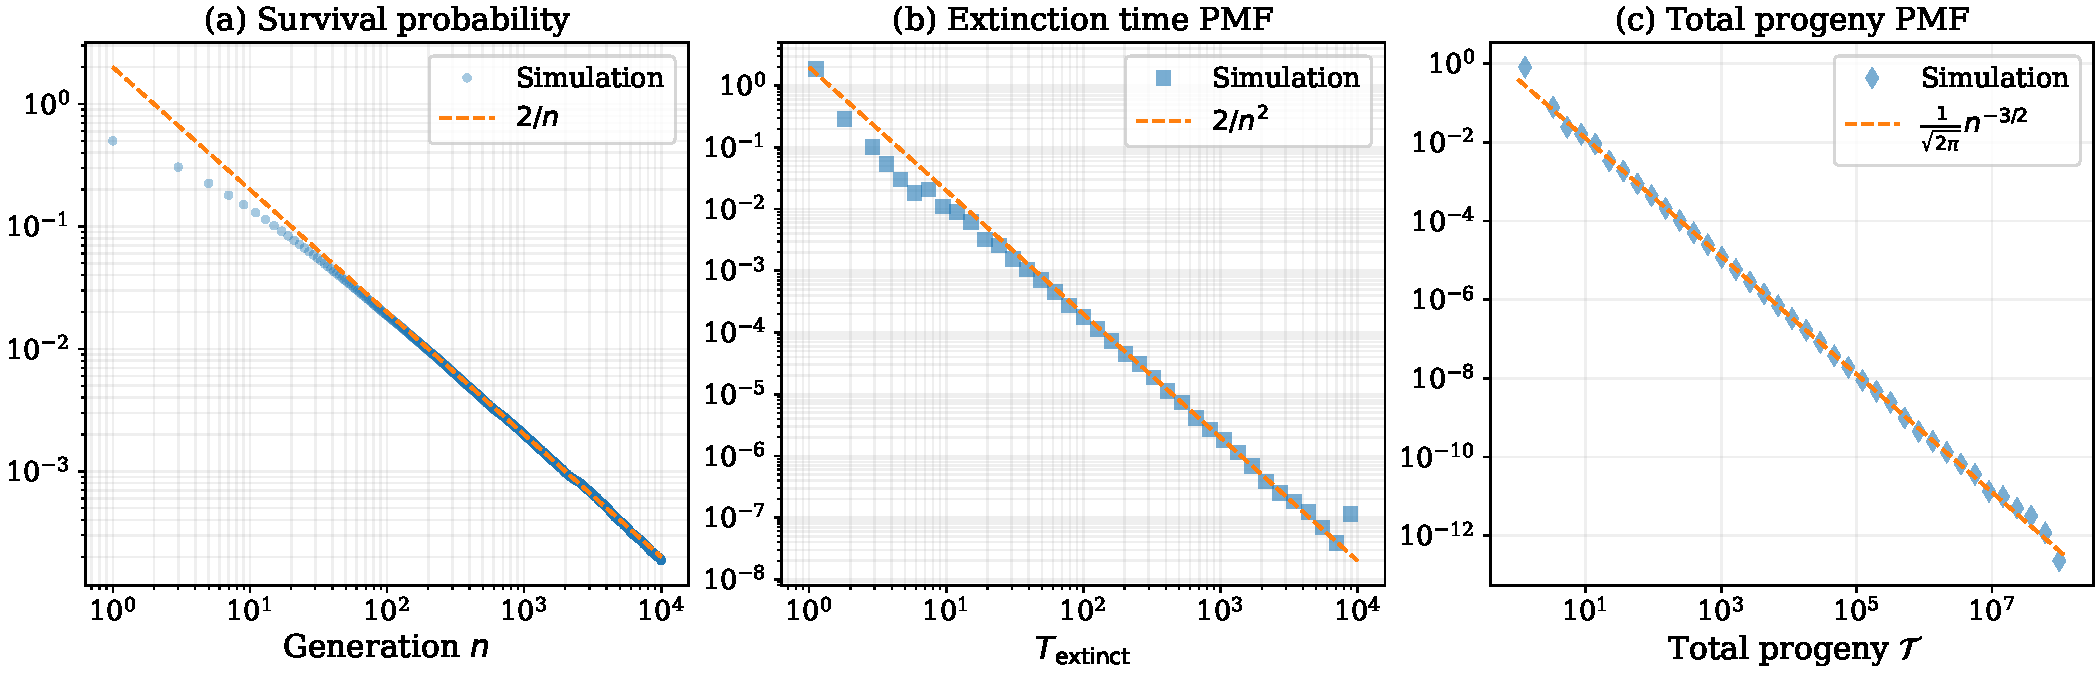
\includegraphics[width=0.98\textwidth]{figures/IMG_ch3/power_law_fixed.pdf}
    \caption{Power-law behaviour at criticality, $p=0.5$, from $10^6$ simulated
    realisations. (a) Survival probability $S_n=\pr{\zz_n>0}$, showing the
    late-generation scaling $S_n\sim2/n$ of \cref{eq:twoovrn}. (b) Probability mass
    function of the extinction time $T=\inf\{n:\zz_n=0\}$, with heavy tail
    $\pr{T=n}\sim2/n^2$. (c) Probability mass function of the total progeny
    $\mathcal{T}=\sum_{k\ge0}\zz_k$, displaying the classical critical branching
    asymptotic $\pr{\mathcal{T}=n}\sim n^{-3/2}$.}
    \label{fig:power_law}
\end{figure}

Criticality is thus the boundary at which the mean stops being informative in either
direction. Below it the population is doomed and the mean says so; above it the
population may establish itself and the mean says roughly how fast. At $p=\tfrac12$ the
mean is one forever while the process is certain to die, and the only way to recover a
useful statement is to condition on survival. That is the subject of the next section.

\FloatBarrier
